% siminos/xiong/thesis/proposal/tex/done.tex
% $Author: predrag $ $Date: 2021-06-22 07:16:06 -0400 (Tue, 22 Jun 2021) $

\section{Preliminary results}
\label{sec:done}

\subsection{Computing \Fv s by \Ped}
\label{subsec:PE}

\begin{figure}[h]
  \centering
  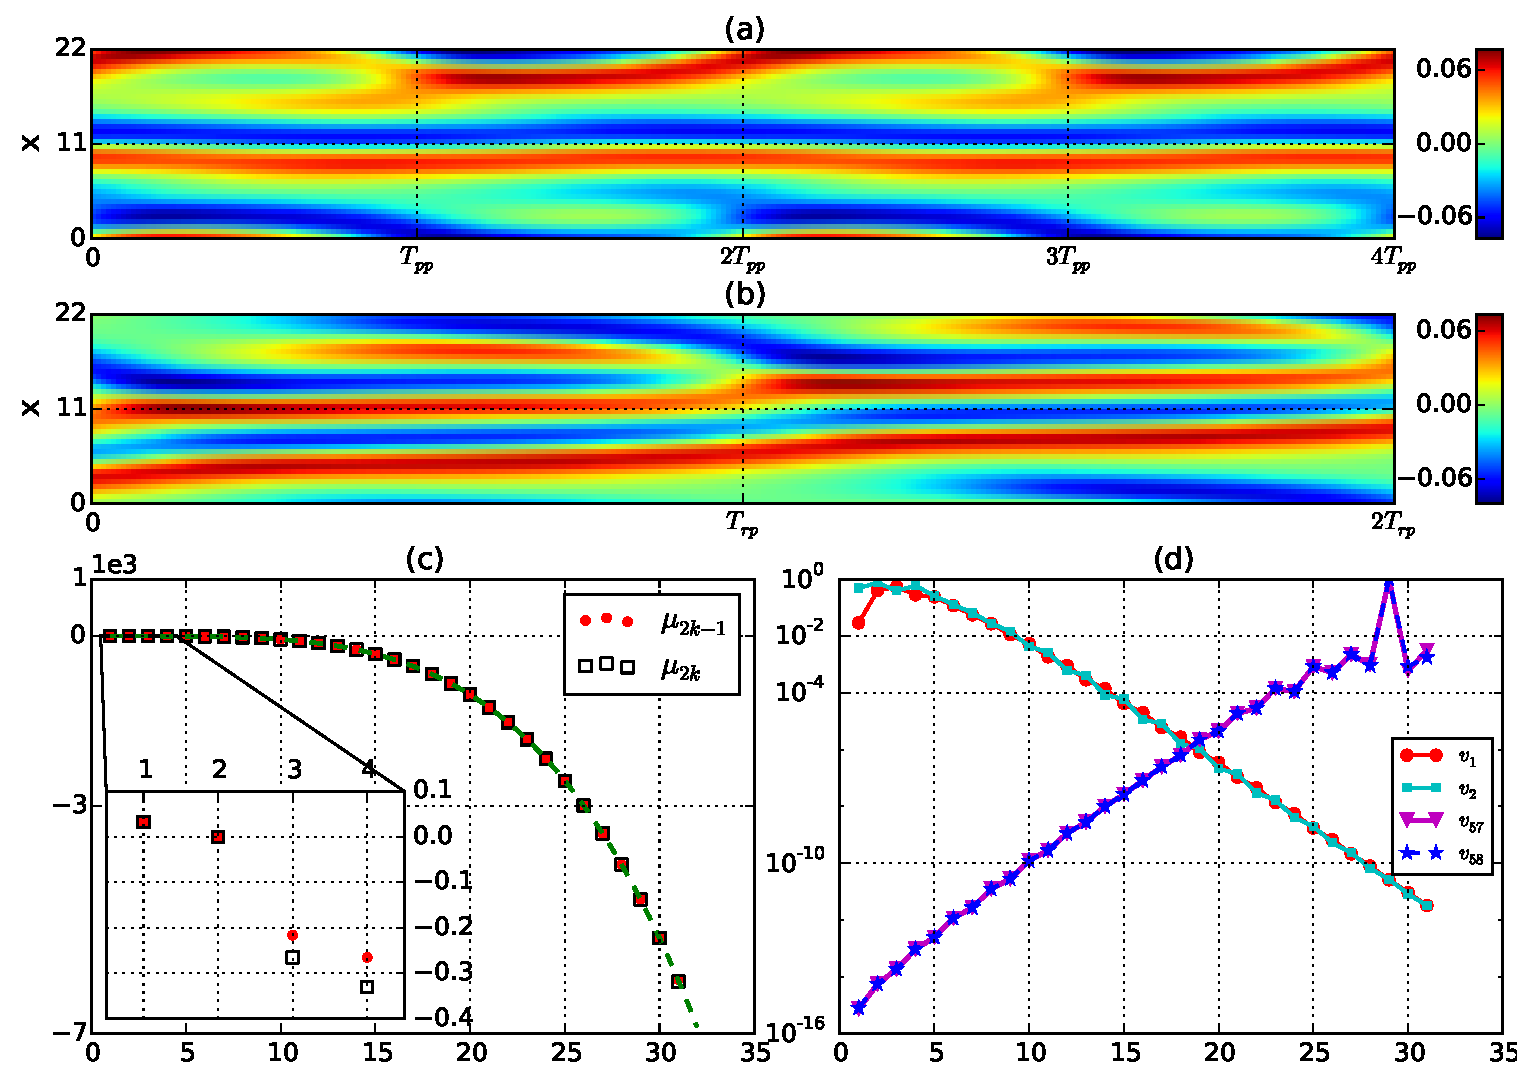
\includegraphics[width=0.9\linewidth]{pprpfigure}
  \caption{(Color online)
   (a) Pre\po\ $\cycle{pp}_{10.25}$ and
   (b) \rpo\ $\cycle{rp}_{16.31}$ in the full \statesp\ for total time
   $4\,\period{pp}$ and $2\,\period{rp}$, respectively. The phase shift
   for $\cycle{rp}_{16.31}$ after one prime period $\simeq-2.863$.
   (c) The real parts of Floquet exponents paired for a given $k$ as
   $(k,\eigRe[2k-1])$ and $(k,\eigRe[2k])$, for $\cycle{pp}_{10.25}$ with
   truncation number $N=64$. The dashed line (green) is
   $q_{k}^{2}-q_{k}^{4}$, with $x$-axis the indices of Fourier modes
   $k=1,2,\cdots,N/2-1$. The inset is a magnification of the region
   containing the 8 leading {\entangled} modes. As can be seen in
   \reftab{tab:floquet_ppo1}, for modes that follow, $k\geq 5$,
   the exponents are much smaller, in
   agreement with the expected separation into {\entangled} and
   {isolated} modes of \refref{YaTaGiChRa08}. For large
   indices, Floquet exponents
   appear in pairs corresponding to the real and imaginary
   part of Fourier modes.
   (d) The magnitudes of the Fourier components $|a_k| =
   |b_k+1i*c_k|$ of the 1st, the 2nd, the 57th and 58th \Fv s
   $\jEigvec[k]$ for $\cycle{pp}_{10.25}$ at initial time $\zeit =0$,
   truncation number $N=64$. For {\entangled} modes the first 4 Fourier
   are comparable in magnitude. For the $k_{th}$ isolated modes pair, the
   amplitude is concentrated on $k_{th}$ Fourier mode. The $x$-axis is
   labeled by the Fourier mode indices. Only the $k>0$ part is shown, the
   negative $k$ follow by reflection.
   }
  \label{fig:ppo1state}
\end{figure}

\begin{table}[h]
  \footnotesize
  \centering
  \caption{
    The first 10 and last four Floquet exponents and
    Floquet multiplier phases,
    $ \ExpaEig_i= \exp(\period{}\,\eigRe[i] \pm i\theta_{i})$, for
    orbits $\cycle{pp}_{10.25}$ and $\cycle{rp}_{16.31}$, respectively.
    $\theta_{i}$ column lists either the phase,
    if the Floquet multiplier is complex, or `-1' if the
    multiplier is real, but inverse hyperbolic. Truncation number
    $N=64$.
    The $8$ leading exponents correspond to the {\entangled} modes:
    note the sharp drop in the value of the $9_{th}$ and subsequent
    exponents, corresponding to the {isolated} modes.
  }
  \label{tab:floquet_ppo1}
  \begin{tabular}{l l c | l l c}
    \multicolumn{3}{c |}{$\cycle{pp}_{10.25}$} & \multicolumn{3}{c}{$\cycle{rp}_{16.31}$}\\
    $i$ & ~~~~~$\eigRe[i]$  & $\theta_{i}$  & $i$ & ~~~~~$\eigRe[i]$ & $\theta_{i}$  \\
    \hline
    1,2 & ~0.033209  &    $\pm$2.0079  &  1 &     ~0.32791  &              \\
    3 & -4.1096e-13  &                 &  2 &   ~2.8679e-12  &              \\
    4 & -3.3524e-14  &    -1           &  3 &   ~2.3559e-13  &              \\
    5 &  -0.21637    &                 &  4 &     -0.13214  &        -1    \\
    6,7 &  -0.26524  &   $\pm$2.6205   &  5,6 &   -0.28597  & $\pm$2.7724  \\
    8 &  -0.33073    &    -1           &  7 &     -0.32821  &       -1     \\
    9 &  -1.9605    &                  &  8 &      -0.36241  &             \\
    10 & -1.9676    &    -1            &  9,10 &   -1.9617  &  $\pm$2.2411 \\
    $\cdots$ &  $\cdots$    & $\cdots$ & $\cdots$ & $\cdots$ & $\cdots$   \\
    59 &  -5313.6   &    -1           &  59 &   -5314.4 &                 \\
    60 &  -5317.6   &                 &  60 &   -5317.7 &                 \\
    61 &  -6051.8   &    -1           &  61 &   -6059.2 &                 \\
    62 &  -6080.4   &                 &  62 &   -6072.9 &                 \\
    \hline
\end{tabular}
\end{table}
\begin{figure}[h]
  \centering
  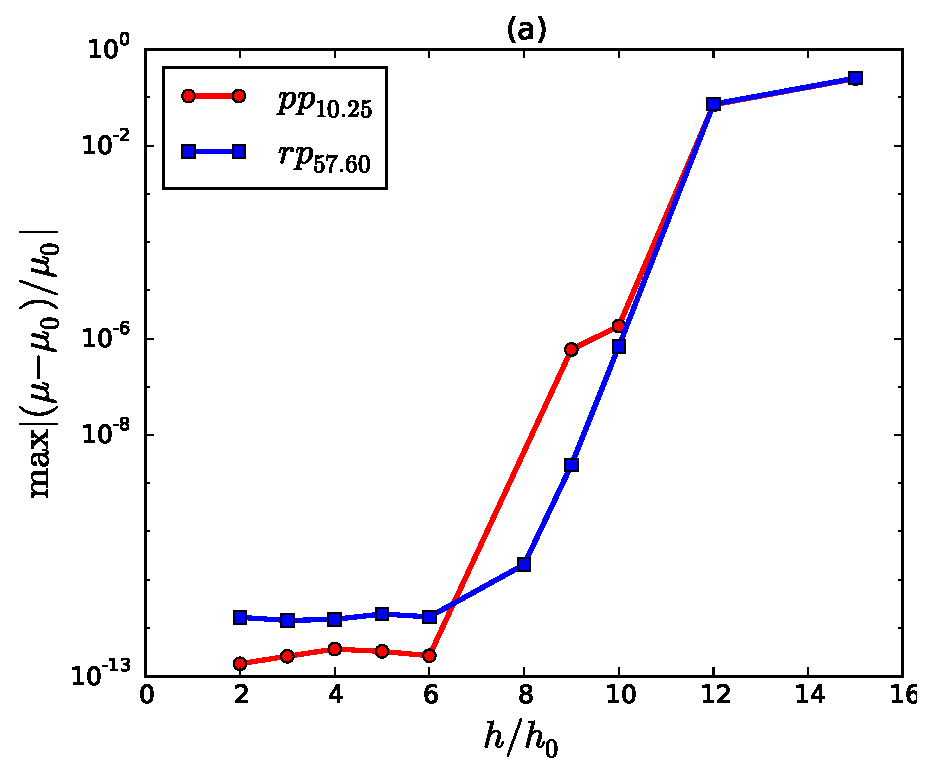
\includegraphics[width=0.47\linewidth]{ppo1FEerror} \hfill
  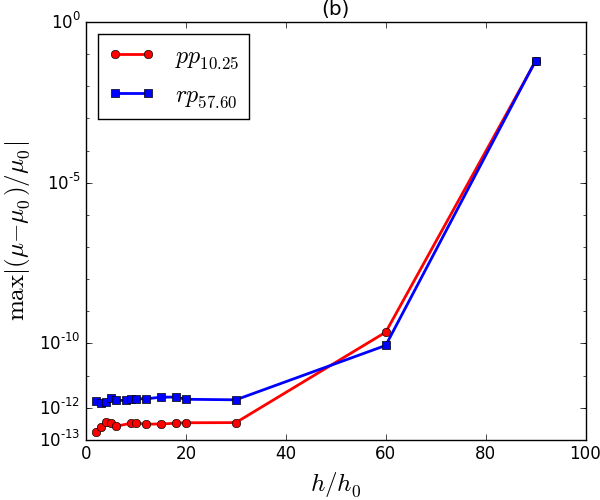
\includegraphics[width=0.47\linewidth]{rpo22FEerror}
  \caption{(Color online) Relative error of the real part of
    Floquet exponents associated with different time steps
    with which the Floquet matrix is integrated. Two orbits $\cycle{pp}_{10.25}$
    and $\cycle{rp}_{57.60}$ are used as an example with the base
    case $h_0 \approx 0.001$. (a) The maximal relative difference of
    the whole set of Floquet exponents with increasing time step (decreasing
    the number of ingredient segments of the orbit). (b) Only consider
    the first 35 Floquet exponents.}
  \label{fig:FEerror}
\end{figure}
\begin{figure}[h]
  \centering
  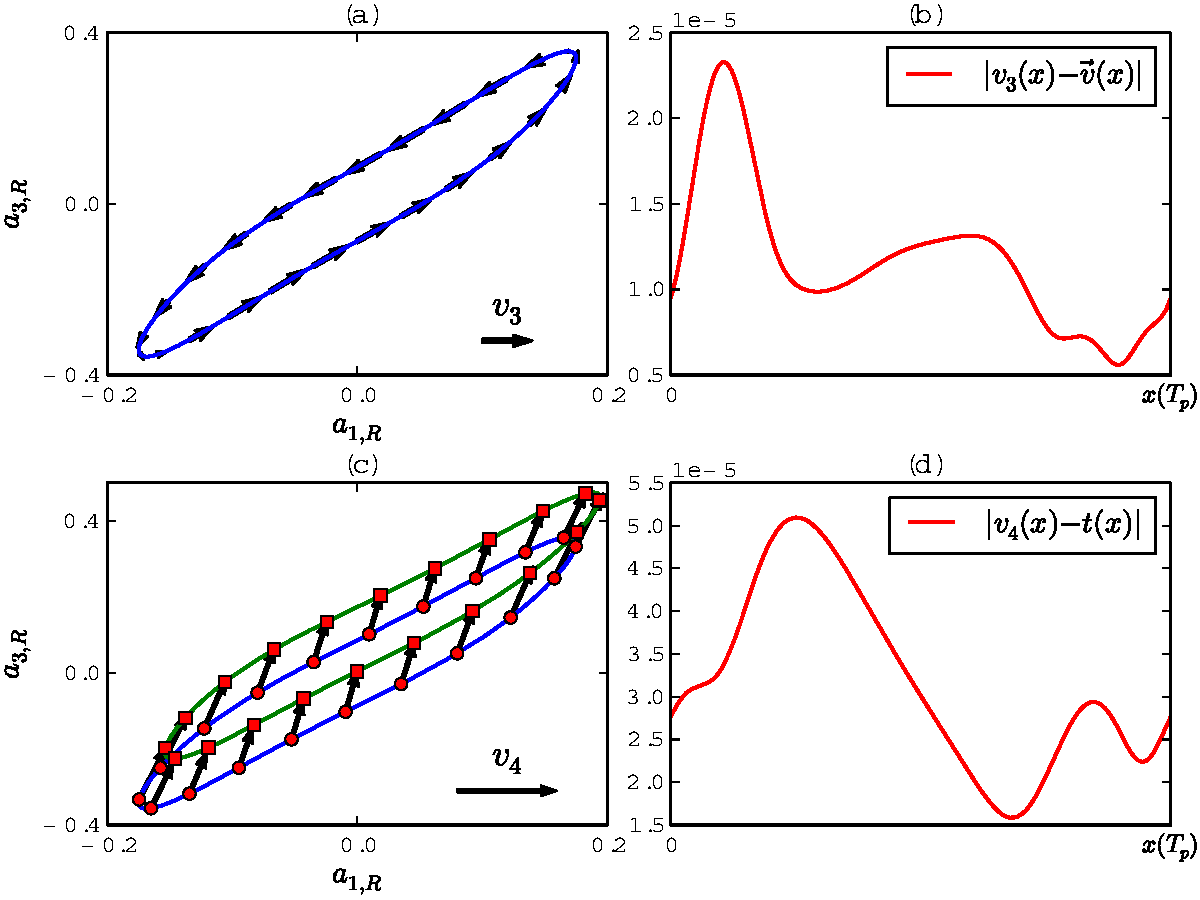
\includegraphics[width=1.0\linewidth]{ppo1vectfield}
  \caption{(Color online)
    Marginal vectors and the associated errors.
    (a) $\cycle{pp}_{10.25}$ in one period projected onto $[a_{1},b_{1},a_2]$
    subspace (blue curve), and its counterpart (green line) generated by
    a small group transformation $g(\ell)$
    , here arbitrarily set to $\ell= \,L/(20\pi)$. Magenta and black
    arrows represent the first and the second marginal \Fv s
    $\jEigvec[3](x)$ and $\jEigvec[4](x)$ along the prime orbit.
    (b) The solid red curve is the magnitude of the difference between
    $\jEigvec[3](x)$ and the velocity field $\vec{v}(x)$ along the orbit,
    and blue dashed curve is the difference between $\jEigvec[4](x)$ and
    the group tangent $t(x)=\mathbf{T}x$.
  }
  \label{fig:ppo1vectorfield}
\end{figure}


Stability analysis of \eqva\ is crucial for understanding the the geometry of
state space\rf{guckb}, but it is difficult for unstable \po s
due to lack of efficient and accurate numerical algorithms.
Floquet theorem says that
the Floquet matrix evaluated along a \po\ can be decomposed
as a product of a periodic matrix and an exponential matrix. We are interested
in the eigenvalues (Floquet multipliers) and the corresponding eigenvectors
(\Fv s) of the exponential matrix. More specifically,
define a flow $x(t) = f^t(x(0))$ generated by velocity field $\dot{x} = v(x)$
with $x$ a state vector. The evolution of perturbation along any orbit
is governed by the Jacobian of this flow
$J^t(x) = \partial f^t(x) / \partial x$, that is
$\delta x(t) = J^t(x) \delta x(0) $, and Jacobian itself is evolved as follows,
\begin{equation}
  \label{eq:jacobian}
  \frac{dJ^t(x)}{dt} = A(x)J^t(x)\,,\quad A(x) = \frac{v(x)}{x}
  \,.
\end{equation}
For a \po\ $x(T_p)=x(0)$,
the solution of \eqref{eq:jacobian}
for one period  $J_p = J^T(x(0))$ is called Floquet matrix or monodromy matrix.
$J_p e_i = e^{T(\eigRe[i]+\eigIm[i])} e_i$ gives the average expansion/contraction
rate $\eigRe[i]$ and
invariant directions $e_i$ in the tangent space.

For high dimensional nonlinear systems, Floquet exponents usually span a large
number of orders, so one period integration of \eqref{eq:jacobian} usually
results in a highly ill-conditioned Jacobian matrix, so we need to conduct
transformations on each short-time Jacobian since whole matrix can be decomposed
into the product of a sequence of square matrix. This is the basic idea of
\emph{\ped}, and it is based on the idea on \cLv\ algorithm and
\psd\ algorithm introduced in sec.~\ref{subsec:CAPSD}. See
\rf{DingCvit14} for the implementation details. Here, we only show the result
with 1-dimensional \KSe\ defined on a periodic domain.
\begin{equation}
u_t+\frac{1}{2}(u^2)_x+u_{xx}+u_{xxxx}=0\,,\; x\in [0,L]
\label{eq:ks}
\end{equation}
Here domain size $L=22$.
\KSe\ is equivariant under reflection and space translation: $-u(-x,t)$ and
$u(x+l,t)$ are also solutions if $u(x,t)$ is a solution.
Based on the consideration of these symmetries,
we focus on two types of orbits:
pre\po s $\hat{u}(0)=R\hat{u}(\period{p})$  and \rpo,
$\hat{u}(0)=g_p\hat{u}(\period{p})$. Here $R$ and $g_p$ are reflection and
rotation respectively.

At each repeat of the prime period, $\cycle{pp}_{10.25}$ is invariant
under reflection along $x=L/2$, \reffig{fig:ppo1state}\,(a), and
$\cycle{rp}_{16.31}$ has a shift along the $x$ direction as time goes on,
\reffig{fig:ppo1state}\,(b). Since $\cycle{pp}_{10.25}$ and
$\cycle{rp}_{16.31}$ are both
time invariant and equivariant under SO(2) group transformation $g(l)$,
there should be two marginal Floquet exponents, corresponding to the
velocity field and group tangent respectively.
\refTab{tab:floquet_ppo1} shows that the $2_{nd}$ and $3_{rd}$,
respectively $3_{rd}$ and $4_{th}$ exponents of $\cycle{rp}_{16.31}$,
respectively $\cycle{pp}_{10.25}$, are marginal, with accuracy as low as
$10^{-12}$, to which the inaccuracy introduced by the error in the closure of
the orbit itself also contributes.

In practice, caution should be
exercised when trying to determine the optimal number of time increments
that the orbit should be divided into. Here we determined satisfactory $m$'s by numerical
experimentation shown in \reffig{fig:FEerror}. Since larger time step means
fewer time increments of the orbit, a very small time step ($h_0 \approx 0.001$)
is chosen as the base case, and it is increased to test whether the
corresponding Floquet exponents change substantially or not. As shown in
\reffig{fig:FEerror} (a), up to $6h_0$ the whole Floquet spectrum varies within
$10^{-12}$ for both $\cycle{pp}_{10.25}$ and $\cycle{rp}_{57.60}$. These
two orbits represent two different types of invariant solutions which have
short and long periods, so we presume that time step $6h_0$ is good enough
for other short or long orbits too. On the other hand, if only the first
few Floquet exponents are desired, the time step can be increased further
to fulfill the job. As shown in \reffig{fig:FEerror} (b), if we are only
interested in the first 35 Floquet exponents, then time step $30h_0$ is small
enough. In high dimensional nonlinear systems, dynamics in the very contracting
directions is, very the often, decoupled from the physical modes, and shed little
insight into the system properties, so large time step could to used in order to
save time.
\refTab{tab:floquet_ppo1} and
\reffig{fig:ppo1state}\,(c) show that \psd\ is capable of resolving
Floquet multipliers differing by thousands of orders:
when $N=64$, the smallest Floquet multiplier  for $\cycle{pp}_{10.25}$ is
$|\ExpaEig_{62}| \simeq e^{-6080.4\times 10.25}$.

The two marginal directions have a simple geometrical interpretation.
\refFig{fig:ppo1vectorfield}\,(a) depicts the two marginal vectors of
$\cycle{pp}_{10.25}$ projected onto the subspace spanned by $[a_1, b_{1}, a_{2}]$
(the real, imaginary parts of the first mode and the real part of the
second Fourier mode). The first marginal eigen-direction (the $3_{rd}$
\Fv\ in  \reftab{tab:floquet_ppo1}) is aligned with the velocity
field along the orbit, and the second marginal direction (the $4_{th}$
\Fv) is aligned with the group tangent. The numerical
difference between the unit vectors along these two marginal directions
and the corresponding physical directions is shown in
\reffig{fig:ppo1vectorfield}\,(b). The difference is under $10^{-9}$ and
$10^{-11}$ for these two directions, which demonstrates the accuracy of
the algorithm.



\subsection{Local description of inertial manifold by \Fv s}
\label{subsec:LDIM}
Dissipative nonlinear systems described by partial differential equations
are infinite dimensional in principle, but for a lot of them, there exists
a finite dimensional inertial manifold and the dynamics is contained in it
after a transient period of evolution. Here we try to explain the concept of
``\emph{slaving}'' to understand how transition from infinite dimensional
space into finite dimensional subspace happens. For strict
mathematical treatment, see\rf{ Robinson1995, infdymnon}. Let $u$ be a dynamical
system in a finite or infinite dimensional Hilbert space $H$ governed by
\begin{equation}
  \label{eq:proto}
  \frac{du}{dt} + Au + f(u) = 0
\end{equation}
Assume this system has a n-dimensional inertial manifold, and
denote the projection from $H$ to the first $n$ eigenvectors of $A$ by
$P$. Let $Q = I - P$, then project \eqref{eq:proto} onto this subspace,
we obtain
\begin{equation}
  \label{eq:projected}
  \frac{dp}{dt} + Ap + Pf(p+\Phi(p)) = 0
\end{equation}
Here $p = Pu$ and $\Phi:PH\mapsto QH$. So we have reduced the dynamics to
a subspace given the existence of such a mapping $\Phi$, and the graph
of $\Phi$ is the inertial manifold. Equation \eqref{eq:projected} is
called the \emph{inertial form} of this system. Essentially, the existence
of inertial manifold indicates that the eigenmodes of $A$ with index larger than
$n$ is slaved to its first $n$ eigenmodes. For example, in \KSe,
eigenmodes of $A$ are Fourier modes, so short waves are slaved to long waves.
Anyway, inertial manifold can be interpreted in different ways, but the essential
idea is similar. See\rf{man90b} for an adiabatic illustration by a simple two
variable system.

To Approximate inertial manifold, or equivalently, to approximate
mapping $\Phi:PH\mapsto QH$ requires the knowledge of its exact dimension.
At present, people use empirical or some test number to truncate the
original system. For example, in \rf{foias88}, 3 modes are
used to represent the inertial manifold of 1-dimensional \KSe, but this
truncated model is not enough to preserve the bifurcation diagram. On the other
hand, mathematical upper bound for the dimension is not always tight.
However, as stated in
sec.~\ref{subsec:IM}, Recent progress in the numerical algorithm of \cLv s enables us
to expand tangent spaces into invariant subspaces.
\CLv s computed along long ergodic
trajectories are disentangled between the physical subspace and the transient
subspace, which serves as a criteria for determining the effective dimension
of the state space. This approach is different from the nonlinear Galerkin method
since it has no ambition to use a static set of eigenvectors to describe the dynamics,
it uses invariant vectors in the tangent space to linearly approximate the
inertial manifold locally.
From our intuition, we expect \Fv s along \po s can give the same dimension
of inertial manifold as \cLv s. Moreover, \Fv s seem more suitable for this job.
First, we have an efficient and accurate algorithm for calculating \Fv s
introduced in sec~\ref{subsec:PE}, and do not
need to follow an ergodic trajectory for a long time as \cLv\ algorithm does.
Second, \po s are dense on the strange attractor and probably only a
small subset of them is enough to represent the whole hierarchy in the system
if the symbolic dynamics of this system is known, so
experiments can be restricted to small number of short \po s.
But \cLv s along ergodic trajectories reveals little information about the
geometry of the strange attractor.


\paragraph{Angle distribution between physical and transient subspaces}
Like the experiments conducted in\rf{TaGiCh11, YaTaGiChRa08}, we measure the
angle between subspaces spanned by disjoint \Fv s along \po s inside
the 1-dimensional \KSe\ with domain size $L=22$.
Since symbolic dynamics in this system is unknown, we choose to do the statics
for all the \po s available to us with period $T<120$.
\begin{figure}[h]
  \centering
  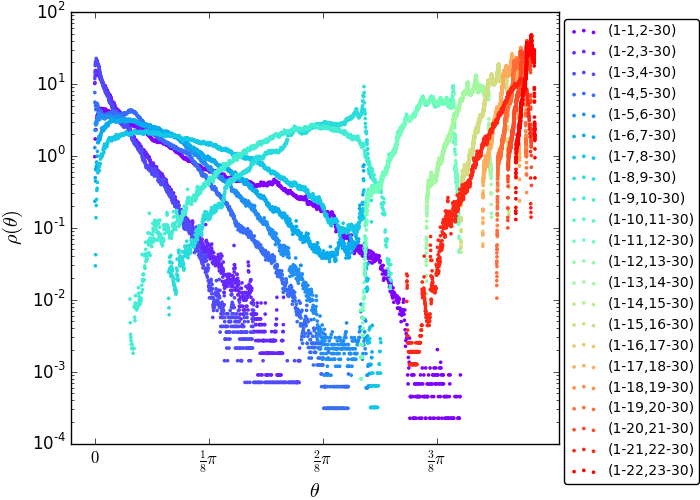
\includegraphics[width=0.48\textwidth]{angle120ppoSpace1} \hfill
  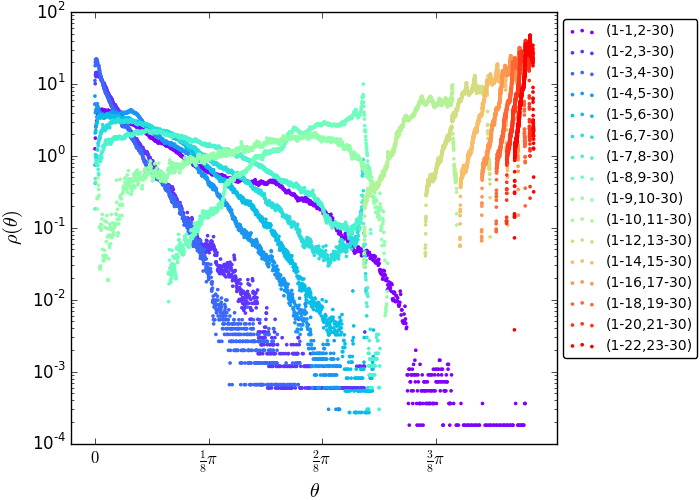
\includegraphics[width=0.48\textwidth]{angle120rpoSpace1}
  \caption{Angle distribution $\rho(\theta)$ versus $\theta$
    for \cycle{ppo} (left) and \cycle{rpo} which has $ T < 120$.
  }
  \label{fig:angDist}
\end{figure}
As shown in \reffig{fig:angDist}, we are measuring the distribution of
the angle between invariant subspace spanned by the first $k$ \Fv s
and the subspace spanned the
remaining $30-k$ \Fv s. Start from $k=1$, As we add more into
the first subspace, the possibility keeps nonzero until $k = 9$, and after
which, the distribution shrinks away from zero. The same qualitative
distribution is obtained for both pre-\po s and \rpo s.
Therefore, the first 8 \Fv s are entangled with each other and are
disentangled from the remaining set. We call the first set physical
\Fv s and the latter unphysical one. The unphysical set has little effect
on the dynamics in the neighborhood of this \po\ since all theses directions
are contracting, and thus small perturbation inside it will die out eventually.
So clearly, the first 8 \Fv s are enough to approximate the inertial manifold
at the neighborhood of all the \po s concerned in this
experiment and we expect that such threshold number
will not
change if we can find more \po s.
Since \po s are dense on the attractor, we expect the same number
apply to the whole inertial manifold.

\paragraph{difference vectors spanned by subset of \Fv s}
Ergodic trajectories are attracted by \po s along their stable directions,
and repelled by their unstable directions. Each unstable direction is
important since it determines how the system is stretched; however, if the
inertial manifold exists, then only a subset of the stable directions
have an effect on the dynamics asymptotically. So we believe that an ergodic
trajectory is moving in a subspace which is spanned by the set of
all unstable \Fv s and a subset of stable \Fv s around a \po\ locally.
So, the number of \Fv s used to span such a subspace can be regarded
as the dimension of inertial manifold.
\begin{figure}[h]
  \centering
  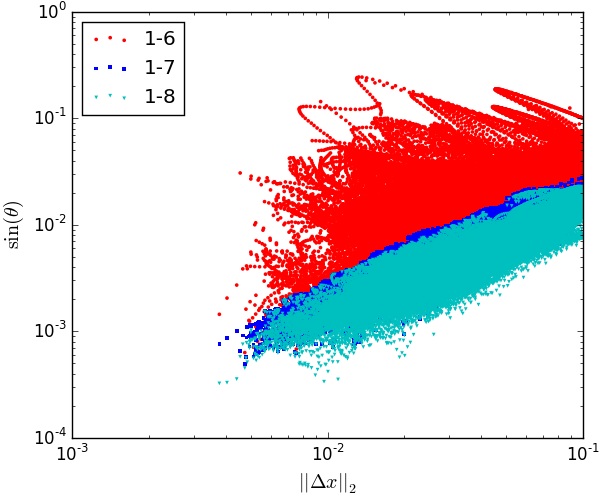
\includegraphics[width=0.48\textwidth]{ppo3truncated} \hfill
  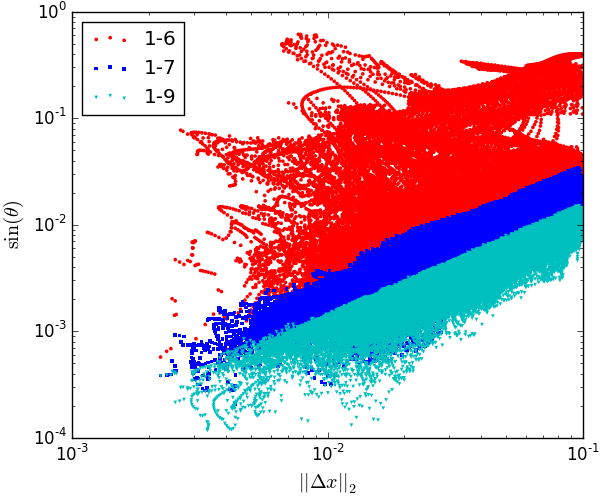
\includegraphics[width=0.48\textwidth]{rpo4truncated}
  \caption{
    scatter plot of $sin\theta$ vs the norm of difference vector.
    $\theta$ is the angle between $\Delta x$ and the subspace spanned
    by a subset of \Fv s.
    (a) $\cycle{ppo}_{32.36}$ with 198 shadowing incidences.
    (b) $\cycle{rpo}_{34.64}$ with 230 shadowing incidences.
  }
  \label{fig:angApproach}
\end{figure}

We borrow the idea from\rf{YaRa11} and conduct a set of experiments.
We generate a long ergodic trajectory and try to find incidences that it shadows
a specific \po. For each shadowing point $x$ on the ergodic trajectory,
we locate the nearest point $x_p$ on the \po\ to it and defined the
difference vector by $\Delta x = x - x_p$. When the orbit approaches or leaves the
\po, the difference vector is mainly controlled by the stable and unstable \Fv s,
so if we try to expand $\Delta x$ using a subset of \Fv s and see
how many of \Fv s is enough for a faithful expansion, we could almost get a
faithful approximation of the inertial manifold locally. In
\reffig{fig:angApproach}, if more than 7 \Fv s are used, then the
tendency shows that $\theta$ will
diminish to zero linearly as $\Delta x$ goes to zero, which is not true
if no more than 6 \Fv s are used to span the subspace. Note the experiments are
conducted in the symmetry-reduced state space, so the dimension of inertial
manifold of the full state space is $7+1$, which is consistent with the previous
result.

\subsection{Traveling wave in \cqcGLe}
In \cqcGL\ \eqref{eq:cqcgl1d}, traveling wave (\reqv) is defined as
a solution of
\[
A(x, 0) = e^{i\phi}A(x+ct, t)
\]
which is
\begin{equation}
  a_k(0) = e^{i\omega_\rho t}e^{ik\omega_\tau t}a_k(t)
  \label{eq:travelWaveFourier}
\end{equation}
in Fourier space.
Here $\omega_\rho$ is the velocity in the group tangent of phase
invariance symmetry: $\phi = \omega_\rho t$, and $\omega_\tau= 2\pi/L\cdot c$.
Levenberg-Marquardt algorithm is implemented to solve \eqref{eq:travelWaveFourier}
with random initial conditions. Dozens of {\reqva} are founded and a few
are shown in \reffig{fig:cqcglReqSet}.
Some of them are extensive spanning the whole domain; others are localized.
\begin{figure}[h]
  \centering
   (1)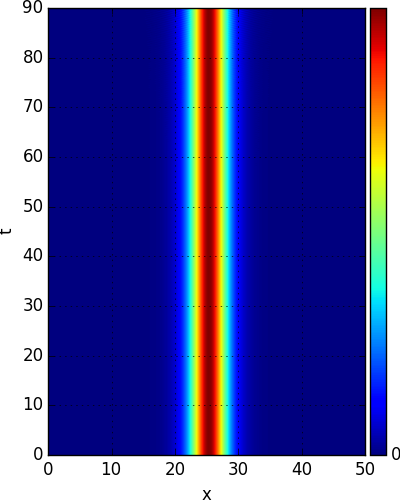
\includegraphics[width=.19\textwidth]{cqcglReq1T90}
   (2)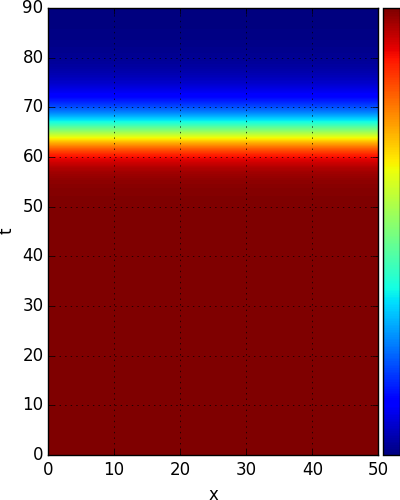
\includegraphics[width=.19\textwidth]{cqcglReq2T90}
   (3)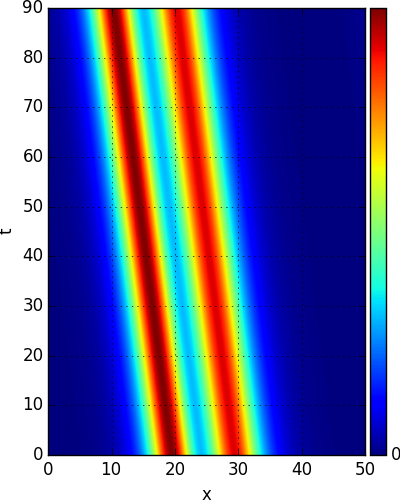
\includegraphics[width=.19\textwidth]{cqcglReq3T90}
   (4)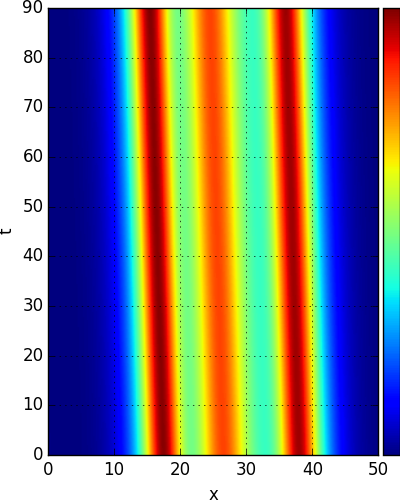
\includegraphics[width=.19\textwidth]{cqcglReq4T90}\\
   (5)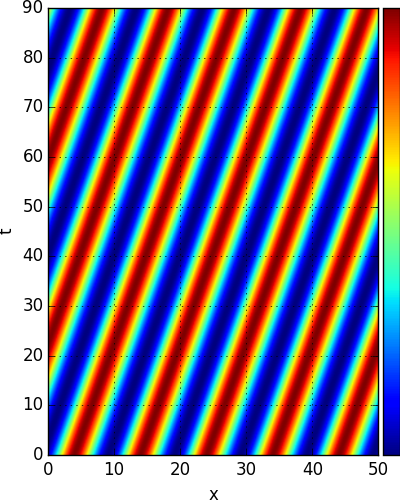
\includegraphics[width=.19\textwidth]{cqcglReq5T90}
   (6)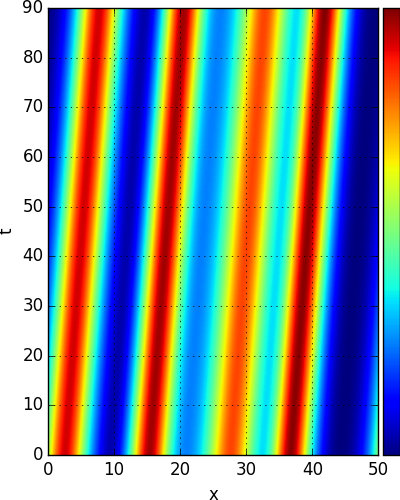
\includegraphics[width=.19\textwidth]{cqcglReq6T90}
   (7)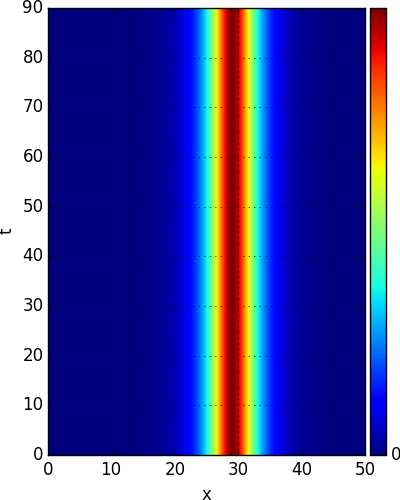
\includegraphics[width=.19\textwidth]{cqcglReq7T90}
   (8)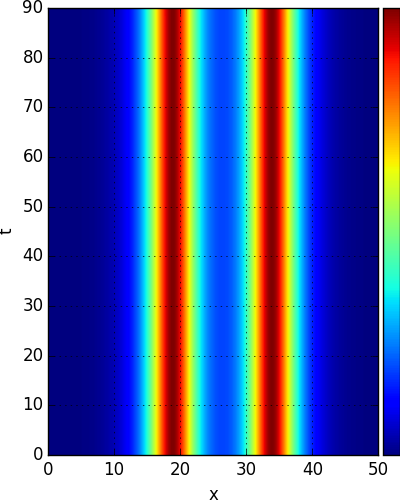
\includegraphics[width=.19\textwidth]{cqcglReq8T90}
  \caption{
    A set of different relative \eqva. (1) is different from
    (7) by the phase velocity. Plane wave solutions like (2) appear
    most frequently, and there is a set of solutions like (2) with
    different phase velocities and translational velocities.
    Only one representative is shown here.
  }
  \label{fig:cqcglReqSet}
\end{figure}
Here I are only interested in the one related to the soliton
(1) shown in
\reffig{fig:req1Config}. This {\reqv} has group velocity
$\omega_\tau = 0$ and $\omega_\rho=17.6675$.
\refFig{fig:req1Config} shows the profile of this \reqv\ and
its stability exponents. \refTab{tab:req1Stability} gives
the numerical values of these exponents.
\begin{table}
  \centering
  \begin{tabular}{c | c}
    index & $\lambda$ \\
    \hline
     1,2    &    0.1474653 $\pm$      17.2375582i\\
     3,4    &    0.1474643 $\pm$      17.2375572i\\
     5    &    -7.21620620e-14             \\
     6    &     -1.86242571e-13  \\
     7,8    &   -0.1002241 $\pm$      17.6645298i\\
     9,10    &   -0.1008975 $\pm$      17.6556189i\\
     \hline
  \end{tabular}
  \caption{The first 10 stability exponents of {\reqv}
   \reffig{fig:req1Config}.
 }
  \label{tab:req1Stability}
\end{table}
\begin{figure}[h]
  \centering
  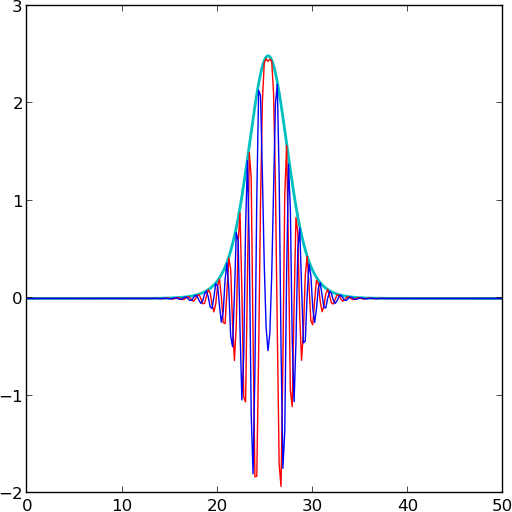
\includegraphics[width=0.35\textwidth]{req1Config} \hfill
  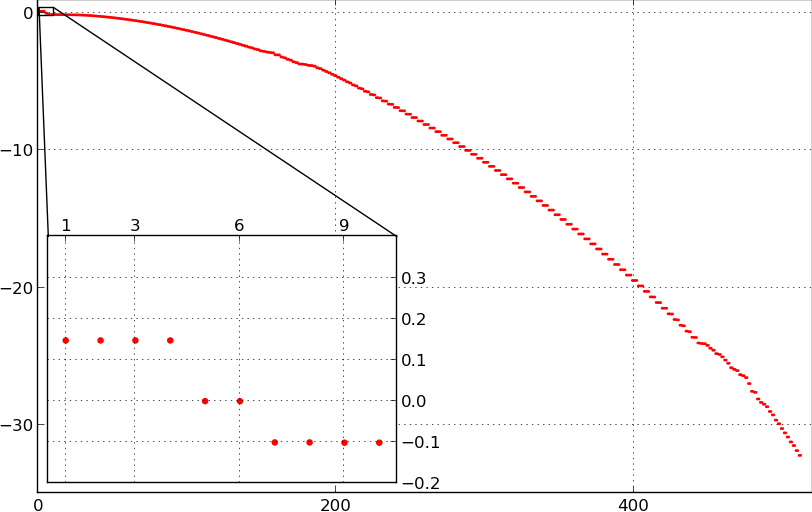
\includegraphics[width=0.55\textwidth]{req1Stability}
  \caption{(Left panel) Spatial profile of the {\reqv} (1) at some
  instant, and the real parts of the spectrum of stability exponents of
  this {\reqv}. The green line is the magnitude of the {\reqv}. Red and
  blue lines are respectively its real and imaginary parts.
  (Right panel) Stability spectrum.
  }
  \label{fig:req1Config}
\end{figure}

There are two marginal directions, which correspond to the group tangents
of translational symmetry and phase invariance. Note the velocity field
lies in this two dimensional subspace.
Four unstable directions are in two conjugate pairs, with almost
the same expansion rates. The corresponding eigenvectors have
almost the same profile.
    \PC{2015-09-06
    We had explained in the blog why exponents come in `almost' quadruplets.
    Is it worth including that here? In any case, that must go into the
    thesis.
    }
Also, the profile is slightly asymmetric
as shown in \reffig{fig:req1eigenvectors}(a)(b).
On the other hand, since
this system has reflection symmetry. The real/imaginary part of the
leading eigenvector of the reflected state is shown in
\reffig{fig:req1eigenvectors}(c)(d). The left side is larger than
the right side for this reflected state.
\begin{figure}[h]
  \centering
  (a)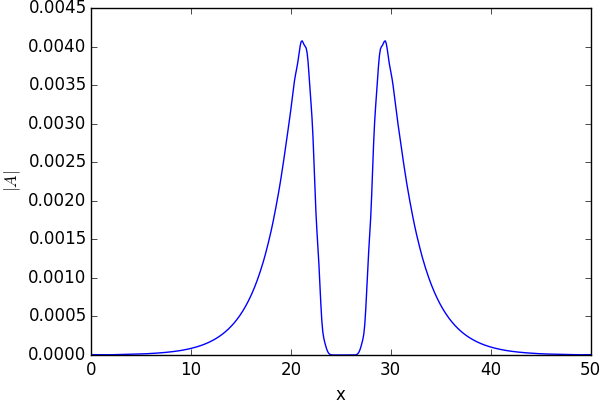
\includegraphics[width=0.46\textwidth]{cqcglReq1V1Real}
  (b)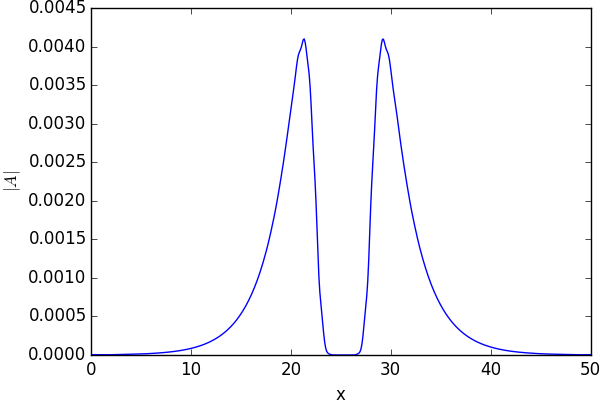
\includegraphics[width=0.46\textwidth]{cqcglReq1V1Imag} \\
  (c)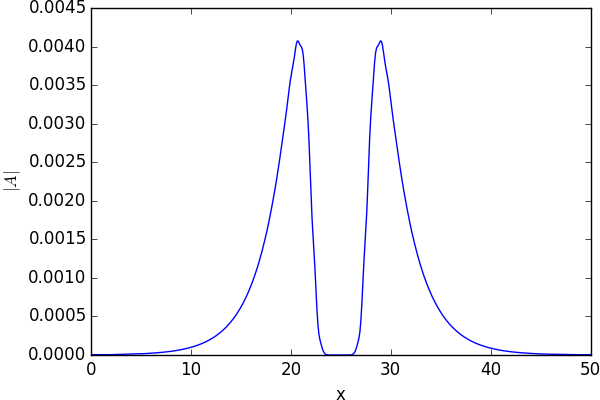
\includegraphics[width=0.46\textwidth]{cqcglReq1ReflectV1Real}
  (d)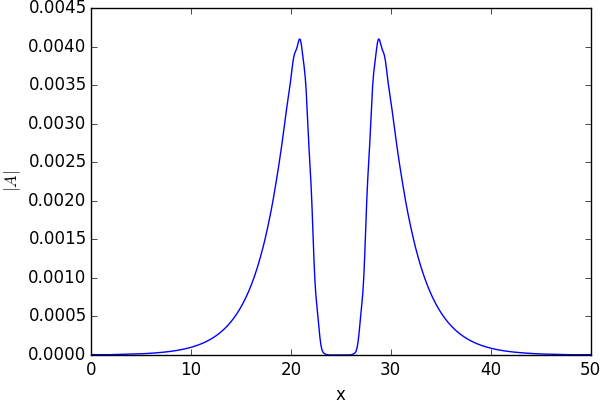
\includegraphics[width=0.46\textwidth]{cqcglReq1ReflectV1Imag}
  \caption{
    Eigenvectors of the {\reqv}.
    (a)(b) the magnitude of the real/imaginary part of the 1st
    eigenvector of the relative equilibrium.
    (c)(d) The relative equilibrium is reflected $A(x)\to A(-x)$.
    The magnitude of the real/imaginary part of the 1st
    eigenvector of the reflected relative equilibrium.
  }
  \label{fig:req1eigenvectors}
\end{figure}
Note that the unstable directions have should profile and the
peaks are exactly at the place where explosion
happens. In this sense, explosions are just homoclinic connections of
this {\reqv}.

Actually, \refref{Akhmediev04} uses an approximation method to
approximate the unstable directions, and gets a symmetric and an asymmetric
solutions, which are used to explain the symmetric and asymmetric
explosions. Here we only got 4 slightly asymmetric solutions, but they have
reflection symmetry, which means that if there are perturbations at both
sides of the soliton, then symmetric explosion also could occur. Also
this is a pure numerical result. No approximation is used.

Next, I will investigate the unstable manifold of this {\reqv} to
see how the flow is organized around this \reqv. But before that,
we need to reduce all the symmetries mentioned in sec.~\ref{subsec:cqcgl}
and then work on the symmetry-reduced state space.

\paragraph{Reduce continuous symmetries} The two continuous symmetry
operations in
\cqcGL\ system can be regarded as one Lie group of two generators, since
these two symmetries commute.
$g(\theta,\phi) = g_\tau(\theta)g_\rho(\phi)$ produces translation in
Fourier space as
\beq
a_k(t) \to a_k(t)e^{i(k\theta + \phi)}
\ee{eq:ft}
In order to reduce this continuous symmetry,
we define a subspace on which all points has vanishing imaginary part
of the 1st and -1st modes
\[
Im(a_1) = Im(a_{-1}) = 0
\,,
\]
and transform all points in the full state space to
this subspace by $ \ssp(\tau) = \LieEl(\theta_s, \phi_s) \, \sspRed(\tau)$
with
\beq
\phi_s = \frac{1}{2}(\alpha_{1}+\alpha_{-1}) \,, \quad
\theta_s = \frac{1}{2}(\alpha_{1} - \alpha_{-1}) \,.
\ee{eq:cqcglPhaseAngle}
Here, $\alpha_{\pm 1}$ are the phase angle of $\pm 1$ mode.
Subscript s denotes the specific angle from slice to full state space.

On the other hand, this choice of slice introduces phase wrapping
problem. From \eqref{eq:cqcglPhaseAngle}, when $\alpha_1$ or
$\alpha_{-1}$ is wrapped, namely, jumps $2\pi$ suddenly, $\phi_s$ and
$\theta_s$ jumps $\pi$. Therefore, at this point, trajectory in the
slice is not continuous. More importantly, it also means that we have
introduced another discrete symmetry. Each orbit in the full state space
has 2 corresponding orbits in the slice, which are related by
$g(\pi, \pi)$. You can have a feeling of how well
slice works in \reffig{fig:cqcglReduceSymT75h005}

\begin{figure}[h]
  \centering
  \begin{subfigure}{.23\linewidth}
    \centering
    \captionsetup{justification=centering}
    \caption{}
    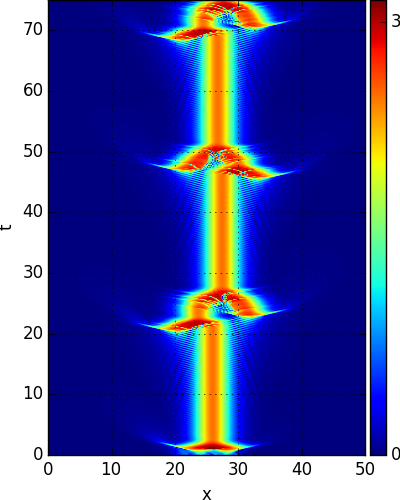
\includegraphics[width=\textwidth]{cqcglStateSpaceT75h005}
    \label{}
  \end{subfigure}
  \begin{subfigure}{.23\linewidth}
    \centering
    \captionsetup{justification=centering}
    \caption{}
    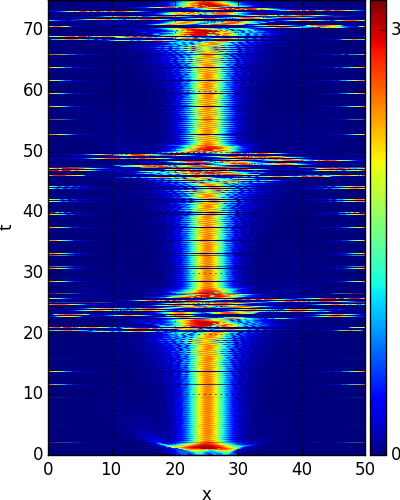
\includegraphics[width=\textwidth]{cqcglSliceWrappedT75h005}
    \label{}
  \end{subfigure}
  \begin{subfigure}{.23\linewidth}
    \centering
    \captionsetup{justification=centering}
    \caption{}
    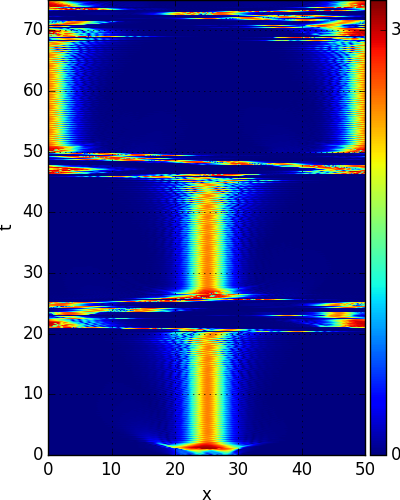
\includegraphics[width=\textwidth]{cqcglSliceUnwrappedT75h005}
    \label{}
  \end{subfigure}
  \begin{subfigure}{.23\linewidth}
    \centering
    \captionsetup{justification=centering}
    \caption{}
    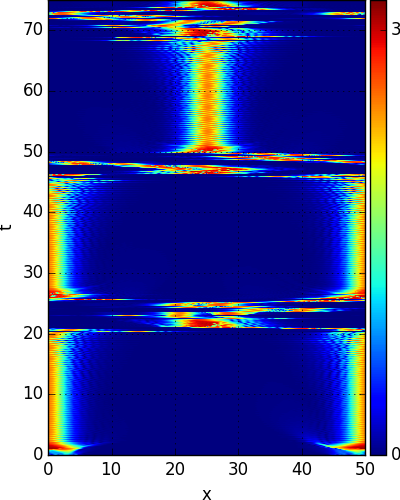
\includegraphics[width=\textwidth]{cqcglSliceUnwrappedShiftedT75h005}
    \label{}
  \end{subfigure}
  \begin{subfigure}{.23\linewidth}
    \centering
    \captionsetup{justification=centering}
    \caption{}
    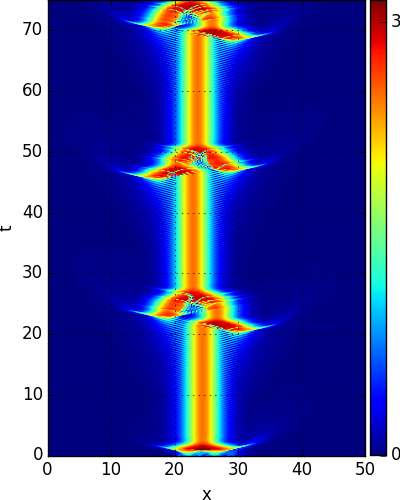
\includegraphics[width=\textwidth]{cqcglStateSpaceReflectT75h005}
    \label{}
  \end{subfigure}
  \begin{subfigure}{.23\linewidth}
    \centering
    \captionsetup{justification=centering}
    \caption{}
    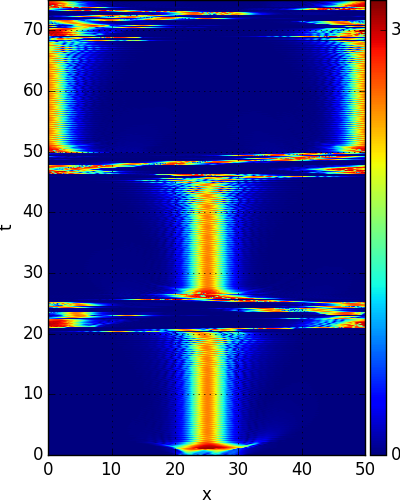
\includegraphics[width=\textwidth]{cqcglSliceUnwrappedReflectT75h005}
    \label{}
  \end{subfigure}
  \begin{subfigure}{.23\linewidth}
    \centering
    \captionsetup{justification=centering}
    \caption{}
    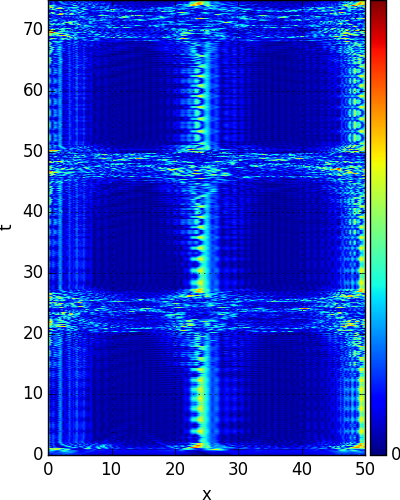
\includegraphics[width=\textwidth]{cqcglAllReduceT75h005}
    \label{}
  \end{subfigure}
  \caption{
    (a) Full state space trajectory.
    (b) Continuous symmetry reduced of (a) with wrapped phase.
    (c) Continuous symmetry reduced of (a) with unwrapped phase.
    (d) rotated by $g(\pi, \pi)$ of (c).
    (e) The reflected states of (a).
    (f) Continuous symmetry reduced of (e).
    (g) after reducing all symmetries of (a)(b).
  }
  \label{fig:cqcglReduceSymT75h005}
\end{figure}


\paragraph{Reduce reflection symmetry}
To illustrate the procedure of reducing reflection symmetry, we'd better split the
real and imaginary part the Fourier modes $a_k = b_k+ 1i*c_k$
and work on the state space defined by
\beq
[b_0, c_0, b_1, c_1, \cdots, b_{N/2-1}, c_{N/2-1},
b_{-N/2+1}, c_{-N/2+1}, \cdots, b_{-1}, c_{-1}]
\,,
\ee{eq:cqcglStateSpace}
Reflection symmetry ($a_k \to a_{-k}$) in state space \eqref{eq:cqcglStateSpace} is
\begin{equation}
(b_0, c_0, b_1, c_1, b_2, c_2, \cdots, b_{-1}, c_{-1})
  \Rightarrow
(b_0, c_0, b_{-1}, c_{-1}, b_{-2}, c_{-2}, \cdots, b_{1}, c_{1})
  \label{eq:reflectFullStateSpace}
\end{equation}
Our strategy is reducing continuous symmetries first, then reducing reflection symmetry.
Inspecting \eqref{eq:reflectFullStateSpace}, you find that
a state point in slice under reflection is still in the slice.
You can analogize it to
the case in a 3-d space: we choose a 2-d plane slice which is perpendicular
to the reflection axis. Therefore, a point in slice will be reflected to another
point in the slice by the original reflection operation. This is the exact reason
for the choice of this specific slice.

Now we try to reduce symmetry \eqref{eq:reflectFullStateSpace}. We take a 3-step
approach. First perform a linear transformation
\begin{align}
& (b_0, c_0, b_1, c_1, b_2, c_2, \cdots, b_{-1}, c_{-1})
  \Rightarrow \nonumber \\
& (b_0, c_0, \frac{b_1-b_{-1}}{2}, \frac{c_1-c_{-1}}{2}, \frac{b_2-b_{-2}}{2},
  \frac{c_2-c_{-2}}{2}, \cdots,
  \frac{b_1+b_{-1}}{2}, \frac{c_1+c_{-1}}{2})
  \label{eq:reflectStep1}
\end{align}
Denote the transformed state as
$(b_0, c_0, p_1, q_1, \cdots, q_{N/2-1}, p_{-N/2+1}, \cdots, p_{-1}, q_{-1})$. So under reflection,
$p_i\,,q_i$ with $i<0$ keep unchanged, but $p_i\,,q_i$ with $i>0$ flip sign. In
the second stage, we perform a nonlinear transformation:
\begin{align}
& (b_0, c_0, p_1, q_1, p_2, q_2, \cdots, q_{N/2-1}, p_{-N/2+1}, \cdots, p_{-1}, q_{-1})
  \Rightarrow \nonumber \\
& (b_0, c_0, r_1, s_1, r_2, s_2, \cdots, s_{N/2-1}, p_{-N/2+1}, \cdots, p_{-1}, q_{-1})
  \label{eq:reflectStep2}
\end{align}
Here $p_i\,,q_i$ with $i<0$ are unchanged.
\[
r_1 = \frac{p_1^2-q_1^2}{\sqrt{p_1^2+q_1^2}}\,,
s_1 = \frac{p_1 q_1}{\sqrt{p_1^2+q_1^2}} \,,
r_2 = \frac{q_1 p_2}{\sqrt{q_1^2+p_2^2}} \,,
s_2 = \frac{p_2 q_2}{\sqrt{p_2^2+q_2^2}} \,,
\cdots
\]
The previous two steps reduce the reflection symmetry of original system
$a_k \to a_{-k}$; however, the specific choice of slice
introduces another reflection symmetry: even modes flip sign.
\begin{equation}
(b_0, c_0, b_1, c_1, b_2, c_2, \cdots, b_{-1}, c_{-1})
  \Rightarrow
(-b_0, -c_0, b_{-1}, c_{-1}, -b_{-2}, -c_{-2}, \cdots, b_{1}, c_{1})
  \label{eq:2ndReflection}
\end{equation}
Under representation \eqref{eq:reflectStep2}, this reflection turns to be
\begin{align*}
& (b_0, c_0, r_1, s_1, r_2, s_2, \cdots, s_{N/2-1}, p_{-N/2+1}, \cdots, p_{-1}, q_{-1})
  \Rightarrow \\
& (-b_0, -c_0, r_1, s_1, -r_2, s_2, \cdots, -r_{N/2-1}, s_{N/2-1},
  p_{-N/2+1}, q_{-N/2+1}, -p_{-N/2+2}, -q_{-N/2+2}, \cdots, p_{-1}, q_{-1})
\end{align*}
Terms $(b_0, c_0, r_2, \cdots, r_{N/2-1}, p_{-N/2+2}, q_{-N/2+2}, \cdots, p_{-2}, q_{-2})$
flip sign, so we can
utilize the same formulation to reduce this reflection symmetry:
\begin{equation}
(b_0, c_0, r_2, \cdots, r_{N/2-1}, p_{-N/2+2}, q_{-N/2+2}, \cdots, p_{-2}, q_{-2})
\Rightarrow
(t_1, t_2, \cdots, t_{N-2})
  \label{eq:reduce2ndReflection}
\end{equation}
\[
t_1 = \frac{b_0^2-c_0^2}{\sqrt{b_0^2+c_0^2}}\,,
t_2 = \frac{b_0 c_0}{\sqrt{b_0^2+c_0^2}} \,,
t_3 = \frac{r_2 c_0}{\sqrt{r_2^2+c_0^2}} \,,
t_3 = \frac{r_3 r_2}{\sqrt{r_3^2+r_2^2}} \,,
\cdots
\]

In conclusion, the following coordinate reduces all symmetries inside
this system.
\begin{equation}
  \label{eq:Finalssp}
  (t_1, t_2, r_1, s_1, t_3, s_2, \cdots, s_{N/2-1}, p_{-N/2+1}, \cdots, p_{-1}, q_{-1})
  \,.
\end{equation}

\refFig{fig:cqcglReduceSymT75h005} (g) shows the state after reducing all symmetries of
this system. When only continuous symmetry is reduced, (a),(e) become (c) and (f) respectively.
Note, (f) is exactly a reflection image of (c). If Reflection symmetries are reduced
further, (c) (d) (f) all turn to (g).
